\section{Introduction}
\label{sec:intro}

% basic introduction to table linking
The World Wide Web is endowed with billions of HTML tables
(i.e. Web tables~\cite{cafarella2008webtables,wang2012understanding}), which carry
valuable structured information. To enable machines to process such tables, or to understand
the web tables, the first step is to link the entities mentioned in the 
tables to a standard lexicon or knowledge base, such as Wikipedia, which 
uniquely identifies entities. This task is
known as entity linking in web tables~\cite{bhagavatula2015tabel,wu2016entity}.
In this paper, we also call it ``table linking''. Because most of the existing
well-known knowledge bases maintain entries primarily in English, much of the table linking
work has been focused on web tables in English~\cite{bhagavatula2015tabel,limaye2010annotating},
hence the techniques developed are for mono-lingual scenarios only.
In reality, the non-English web also possesses many web tables with equally precious information
that would benefit not only people speaking that particular language,
but also the English world.
For example, information extracted from a table about Chinese celebrities can be
used to enrich knowledge in Freebase or IMDB.
On the other hand, since knowledge bases in English are more
comprehensive and accurate than that of other languages,
entity linking systems in foreign languages often fail to identify 
an entity due to incompleteness of KB in their languages.
Incorporating English entities into the target KB can improve 
the recall of entity linking systems in such cases.
%\KZ{The above reason seems not compelling enough to make the following
%claim.}
Therefore, there is a substantial need to link entities in 
non-English web tables
to English knowledge bases. \figref{fig:chinesetable} depicts such a scenario. 
After cross-lingual table linking, ``上海'' in the second row is linked to its 
corresponding real world entity \textit{Shanghai} in a KB (e.g., Freebase).
%\KZ{Change to an example that shows rare entites in Chienese but available in
%English KB.}

\begin{figure}[th]
\centering
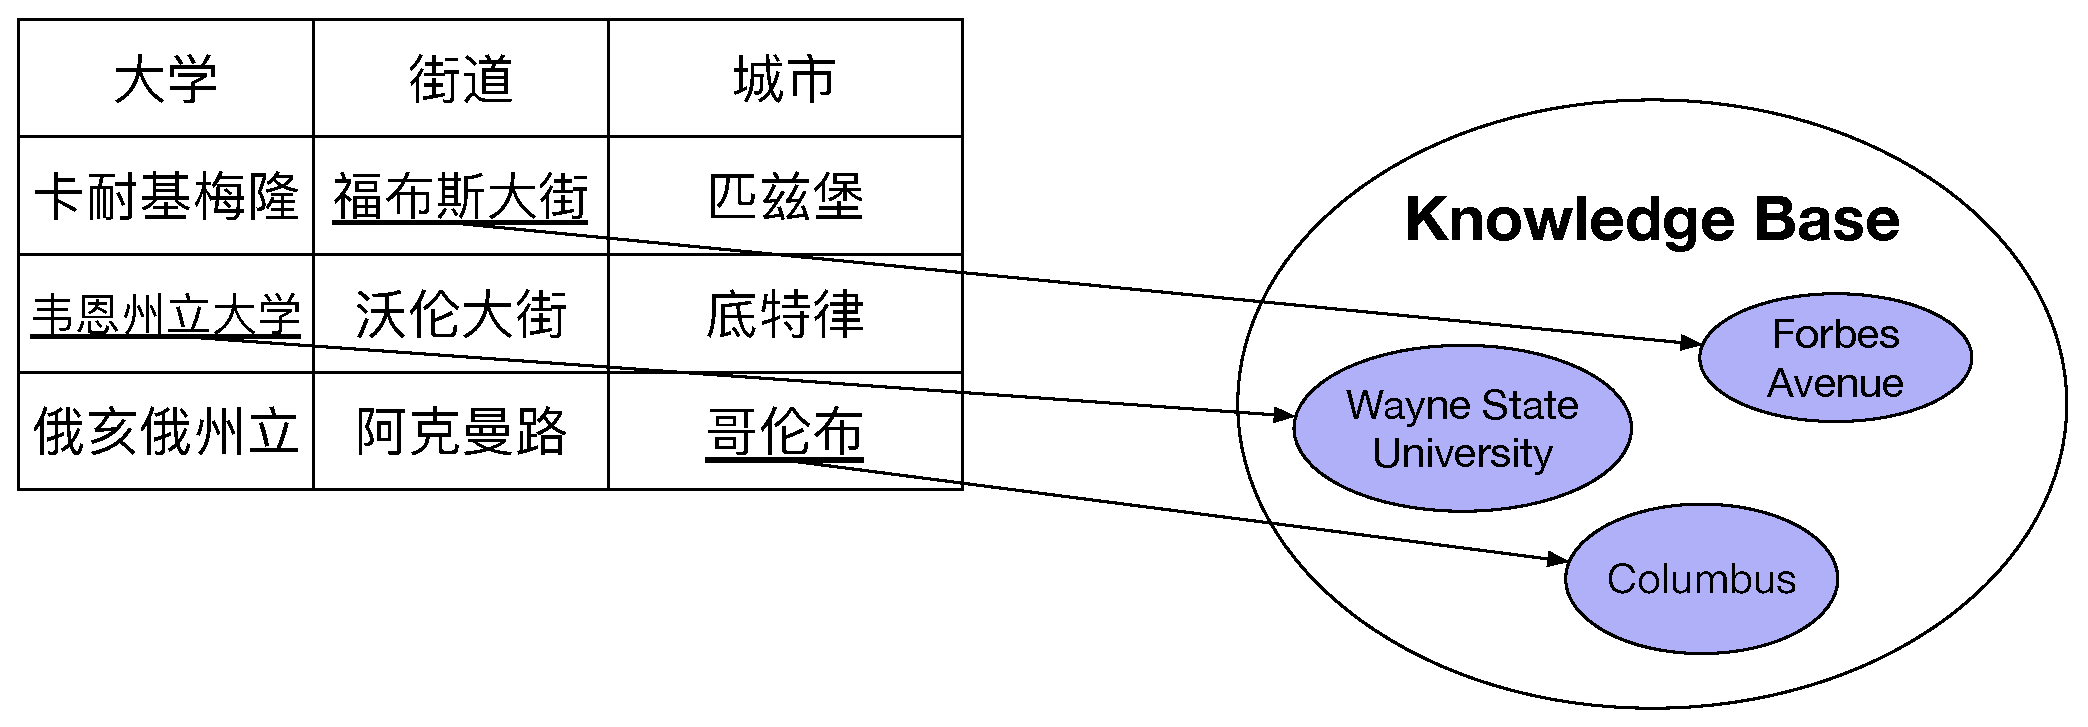
\epsfig{file=intro_example.eps, angle=0, width=1.0\columnwidth}
\caption{Example of Cross-lingual Table Linking from Chinese to English}
\label{fig:chinesetable}
\end{figure}

There are two naive approaches to accomplish this cross-lingual table linking task.
In the first approach, one can use any of the mono-lingual table linking techniques developed thus far
to first link the entities to a knowledge base of that language or culture, and then link to
the English knowledge base via inter-language links~\cite{tsai2016cross}.
For example, Wikipedia is a multi-lingual knowledge base that provides such inter-language links. 
The problem with this approach is that the non-English knowledge base may not be
comprehensive enough to carry all the entities in the web tables in question.
The Chinese Wikipedia, for instance, is only about 1/6 the size of the English
Wikipedia, by the number of articles. Furthermore, many non-English knowledge sources
provide no inter-language links. 

In the second approach, one can directly translate all the entity names in
the non-English web table into English,
and then use the mono-lingual table linking techniques to link to 
an English knowledge base~\cite{mcnamee2011cross}.
This two-step approach is also not effective because
it is analogous to a distant supervised learning, where the association between
non-English names and English entities are not directly available for training. If the translation is not correct, the error will propagate in the following linking steps.


%The key step of converting Web tables into machine-readable knowledge 
%is entity linking, which refers to a task of mapping the mentions in table cells to the referent entities in a Knowledge Base (KB), such as Freebase and Wikipedia. 
% add some example

% However... non-English KB is not good enough, give some examples.
%Most widely used KBs are written in English. KBs in other languages suffer backwards at both size and quality. For example, The latest English Wikipedia contains XXXX articles while Chinese version only has a size of XXXX.\XS{say sth about quality} In the meantime, the percentage of Web pages written in English are decreasing due to widely development of Web technology accross different cultures. Thus, it becomes more and more important to maintain the growth of KBs by absorbing infomation from all Web contexts of different languages. In the previous example, the table could be in a Chinese article so the mention to link  is ``XXX'' instead. We call this new task as cross lingual table linking.

% Challenges, table -> no contexts, language -> gap 
% First try on cross lingual table linking
%There are various efforts \XS{cite} trying to solve entity linking task 
%for Web tables while no one ever makes an attempt under cross lingual environment.

In this paper, we attempt to solve the cross-lingual table linking problem
without the use of any non-English knowledge bases. That is, our goal is to link the mentions in the non-English table directly to an entity in the English knowledge base. 
The advantage of this is we do not discard any information of non-English mentions so that our model has the ability to tolerate the error caused by translation.
To the best of our knowledge, this is the first attempt that attacks the 
cross-lingual table linking problem. 
In all entity linking tasks (mono-lingual or cross-lingual), 
a necessary step in any approach is to generate a set of candidate entities
~\cite{tsai2016cross,mcnamee2011cross,bhagavatula2015tabel,wu2016entity},
and then the problem is transformed to a ranking problem, which aims to pick
the entity that is most similar to the mention in the table. 
The similarity computation requires the feature representation for a mention to be 
compatible with the representation for an entity. 
The major technical challenge of our task is since the source mention
and the target entity come from two difference languages,
their feature representations are naturally incompatible and incomparable. 
To make matters worse, tables offer very limited context for disambiguating
a mention in the first place.

%Since the language of source mention and target entity is inconsistent, 
%it's hard to direct use the surrounding infomation of them \XS{rephrase}. 
%Besides, this task still has to face a lack of surrounding contexts 
%which can be very helpful during entity disambiguation in normal entity linking tasks.

% image CNN, table is like image
We propose a joint model based on neural network for cross-lingual table linking. We embed mention, context and entity in continuous vector space to capture their deep semantics.
Based on that, we employ a linear transformation to do a primary translation between vector spaces of two languages. 
For each table, we link all the mentions simultaneously, in order to fully utilize the relationships among entities in the same row or column. We encode this correlations as a coherence feature in the model.
Furthermore, we design a pairwise ranking loss function for parameter learning and propose an iterative prediction algorithm to link new tables.



%Most existing work \XS{cite} mines hand-crafted features to measure the similarity 
%between mentions and candidate entities.  Since feature engineering suffers XXX, 
%some work attempt to use nerual network \XS{cite} to generate fearures, 
%which shows great improvements in task of entity linking. 
%
%As we should notice, a table can be regarded as a matrix of texts, similar to an image, which is a matrix of pixels. 
%Inspired by that idea of using deep neural networks to capture rich semantics of images, which has been proven successful, 
%we present a jointly modeling framework based on nerual networks to solve our problem.
%Besides, Convolotional Neural Networks(CNN) is a natural structure to deal with data in matrix form such as tables.

% Contribution
The contribution of this paper can be summarized as follows.
\begin{itemize}
\itemsep0em
\item We formally define the problem of cross-lingual entity linking for Web tables (\secref{sec:problem});
\item We present a novel neural network based joint model which effectively captures the rich semantics of mention table and referent entity table simultaneously. Based on that, we bridge the gap between different languages in this task (\secref{sec:approach});
\item We propose a coherence feature in the joint linking model which captures the correlation of entities appearing in the same table and improves the linking accuracy (\secref{sec:coherence});
\item The framework significantly outperforms
several baseline methods, with an accuracy of 63.6\%. (\secref{sec:eval}).
%and question answering. Furthermore, our schema representation is
%on par with the popular word embedding model in computing relation similarity (\secref{sec:eval}).
\end{itemize}
